\documentclass[../main.tex]{subfiles}

\graphicspath{{../images/}}

\begin{document}
\pagestyle{fancy}
\lhead{Module 2}
\chead{Junseo Shin}
\rhead{CSE 4059}

\section{Module 2}

\subsection*{Vector Add}

\begin{figure}
    [ht]
    \centering
    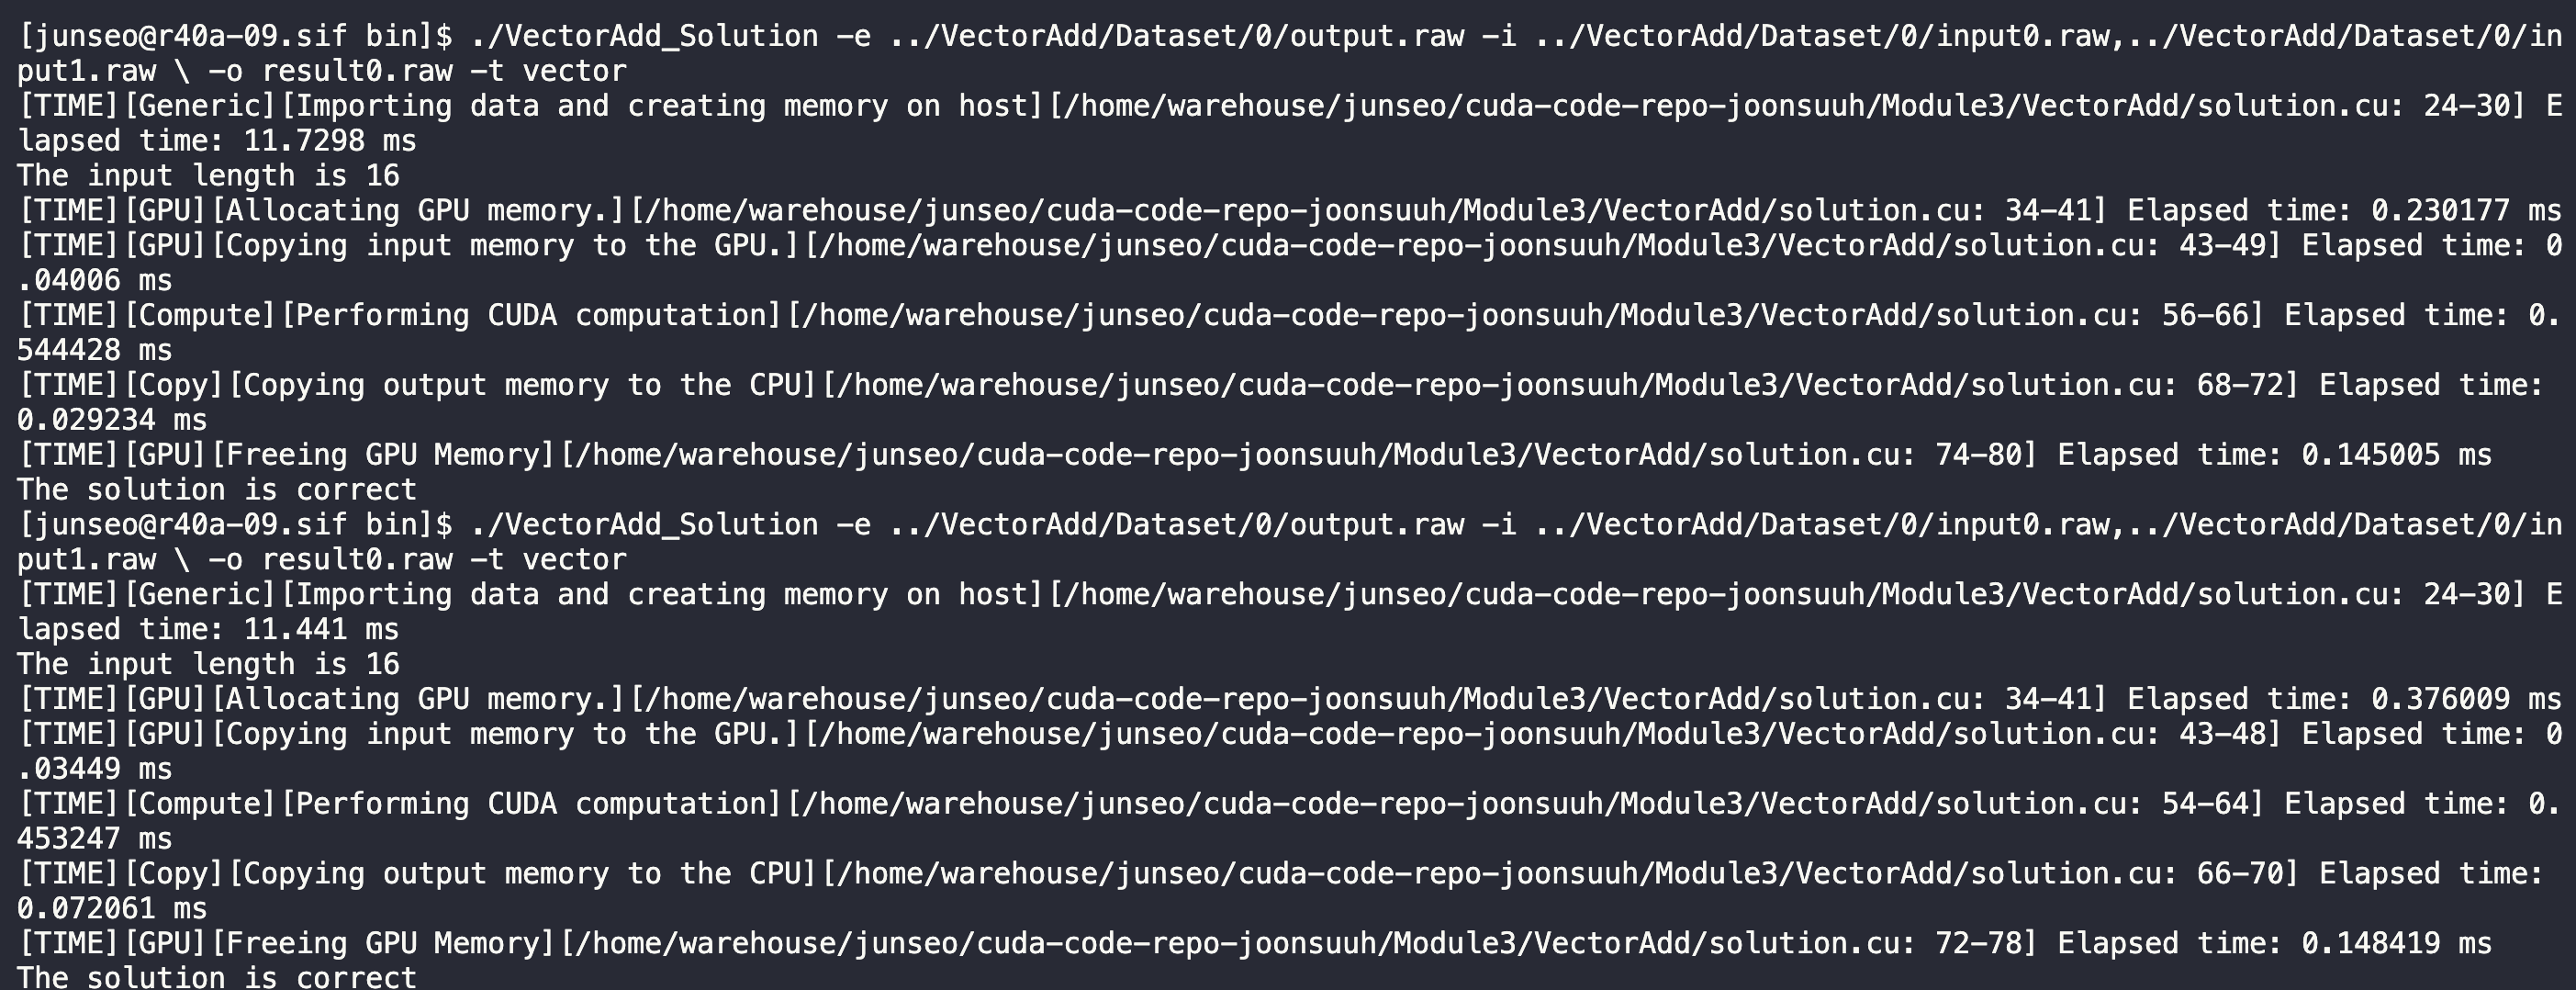
\includegraphics[width=0.8\textwidth]{vectoradd.png}
    \caption{\texttt{Vector\_Add\_Solution} output}
\end{figure}

\subsection*{Questions}

\begin{enumerate}
    \item How many floating operations are being performed in your vector add
    kernel? EXPLAIN.

    

    \item How many global memory reads are being performed by your kernel?
    EXPLAIN.
    
    \item How many global memory writes are being performed by your kernel?
    EXPLAIN.
    
    \item Describe what possible optimizations can be implemented to your kernel
    to achieve a performance speedup.
    
    \item Name three applications of vector addition.
\end{enumerate}



\end{document}